\documentclass[border=2pt]{standalone}
\usepackage{fontspec}
\setmainfont{Liberation Serif}
\usepackage{tikz,graphicx,pgfplots}
\usetikzlibrary{arrows.meta,positioning,matrix,calc}
\pgfplotsset{compat=1.18}
\definecolor{forest}{HTML}{176044}
\definecolor{sage}{HTML}{EAF4EE}
\definecolor{rulec}{HTML}{CBD4CF}
\definecolor{ink}{HTML}{192723}
\definecolor{warm}{HTML}{F3ECE4}
\tikzset{all/.style={font=\fontsize{10.5pt}{12.5pt}\selectfont,text=ink},
box/.style={all,draw=rulec,fill=sage,rounded corners=2pt,align=center,inner sep=4pt,minimum height=0.9cm},
mutedbox/.style={box,fill=white},warmbox/.style={box,fill=warm},
flow/.style={-{Latex[length=2.4mm]},line width=.65pt,draw=forest}}
\begin{document}
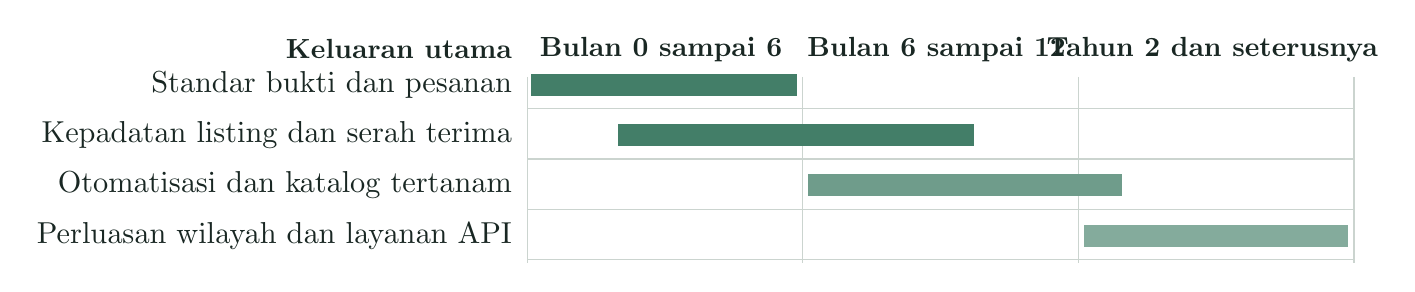
\begin{tikzpicture}[x=1cm,y=1cm]
\node[all,anchor=east,font=\fontsize{10.4pt}{12pt}\selectfont\bfseries] at (4.58,.45) {Keluaran utama};
\foreach \x/\label in {6.35/{Bulan 0 sampai 6},9.85/{Bulan 6 sampai 12},13.35/{Tahun 2 dan seterusnya}} {
\node[all,font=\fontsize{10.2pt}{12pt}\selectfont\bfseries] at (\x,.45) {\label}; }
\foreach \y/\label in {0/{Standar bukti dan pesanan},-.64/{Kepadatan listing dan serah terima},-1.28/{Otomatisasi dan katalog tertanam},-1.92/{Perluasan wilayah dan layanan API}} {
\node[all,anchor=east] at (4.58,\y) {\label};
\draw[rulec] (4.65,\y-.305)--(15.15,\y-.305);
}
\foreach \x in {4.65,8.15,11.65,15.15}{\draw[rulec] (\x,.10)--(\x,-2.27);}
\fill[forest!81] (4.70,-.14) rectangle (8.08,.14);
\fill[forest!81] (5.80,-.78) rectangle (10.32,-.50);
\fill[forest!62] (8.22,-1.42) rectangle (12.20,-1.14);
\fill[forest!53] (11.72,-2.06) rectangle (15.08,-1.78);
\end{tikzpicture}
\end{document}
